\documentclass[a4paper]{article}

\usepackage{amsmath}
\usepackage{amsfonts}
\usepackage{amssymb}
\usepackage[pdftex]{graphicx}
\usepackage[spanish]{babel}

\begin{document}

\begin{center}

\begin{center}
\includegraphics[scale=0.5]{Logo.PNG} 
\end{center}
\hspace{20pt}

\huge
\textbf{Ingeniería básica de una caldera bagacera}\\ 
\hspace{50pt}

\Large
Tema de Trabajo Profesional - Rama Termomecánica\\ 

\hspace{10pt}

\large
\textit{Tutor: Ing. Pablo Barral}\\

\small
67.33 Tecnología del Calor\\

\hspace{8pt}

\small  
\texttt{pbarral@fi.uba.ar}\\

\end{center}

\hspace{8pt}

\begin{center}
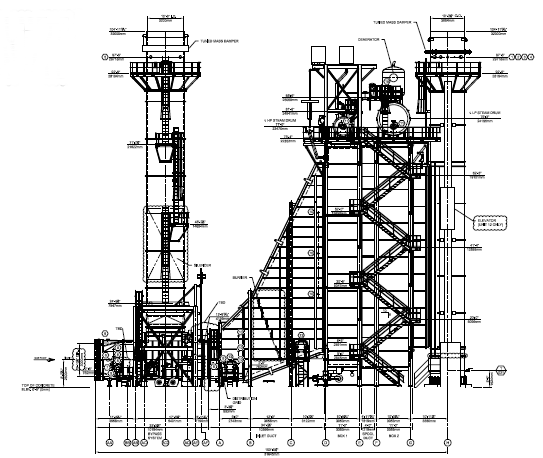
\includegraphics[scale=0.45]{Captura.PNG} 
\end{center}
\hspace{8pt}

\begin{flushright}
\textit{\today}
\end{flushright}

\newpage
\normalsize

\section*{Objetivo}

El propósito de este trabajo es estudiar el funcionamiento y la documentación de la librería de Python "TESPy".\footnote{Esta librería de código abierto permite simular sistemas térmicos tales como ciclos de Joule-Brayton, ciclos de Rankine, ciclos frigoríficos, etc.}

Se estipula realizar este estudio mediante la implementación en Python de un ciclo de cogeneración consistente en dos turbinas de gas con sendas calderas de recuperación y una turbina de vapor a extracción-condensación.

A partir de este desarrollo se desea efectuar una validación propia de la librería contra el benchmark formado por el ciclo elegido, del cual se poseen los datos reales simulados por los fabricantes de los equipos.

Finalmente, como objetivos secundarios podemos mencionar:
\begin{enumerate}
    \item incorporar a la documentación un ejemplo que la complete,
    \item llevar a cabo un análisis exergético del ciclo elegido, utilizando la funcionalidad incorporada en la librería,
    \item generar un trabajo que pueda ser, con ciertos retoques y adecuaciones, eventualmente publicable, y
    \item arribar a un trabajo que pueda continuarse por otro grupo en el futuro, mediante la incorporación de complejidad al modelo.
\end{enumerate}

\section*{Justificación}

Este trabajo surge de la problemática a nivel mundial en el área, donde los software especializados\footnote{Thermoflow, CycleTempo, Ebsilon, etc.} son extremadamente onerosos y, por lo tanto, inaccesibles para la academia y para los estudios de ingeniería, los cuales son responsables de buena parte de la innovación y el desarrollo en el área. Esta problemática figura en los trabajos citados en la bibliografía, y es la que motivó al programador a emprender el desarrollo de una herramienta de código abierto.

Es por esto que la librería TESPy está bien documentada y tiene resultados publicados (los cuales validan su aplicabilidad). Sin embargo, ni en la documentación ni en los artículos se encuentra como ejemplo una cogeneración como la que se propone este trabajo. Esto es esperable, ya que los tipos de cogeneración que son más comunes en Europa (lugar de origen del desarrollador y de su medio académico) son distintos a los que se requieren en países como Argentina (con una demanda sostenida y significativa de energía térmica derivada de la agroindustria). El modelo propuesto para el estudio pertenece a esta última clase.

Se pretende estudiar esta librería porque permite automatizar aspectos que hoy se llevan a cabo, en el medio local, a mano en EES. Esta automatización habilita a poder contar con simuladores más robustos y con mayor flexibilidad para realizar cambios y para hacerlos a mayor velocidad.\footnote{Por ejemplo, serviría para trabajos profesionales como el del simulador de ciclo Rankine, el del estudio termoeconómico de uno de estos ciclos o como el del aprovechamiento energético.}. Además, al ser de código abierto, permite una auditoría transparente de los resultados a los que se arriban. Todo esto contribuye a que sea una herramienta que colabore para la implementación de estudios de eficiencia y de performance de ciclos en un entorno industrial.

Para poder hacer esto, antes de la adopción se requiere un estudio exhaustivo de las capacidades de la librería. Esta tarea puede encomendarse a un aspirante a ingeniero mecánico. Este estudio puede llevarse a cabo mediante un ciclo como el propuesto, ya que es completo, al incluir equipos diversos y contarse con datos de la performance en distintos modos de operación.

Además de su factible utilización en un entorno industrial, esta librería tiene, por su modularización, potencial para implementarse en la docencia, lo que permitiría aumentar en gran medida los ejemplos expuestos en Tecnología del Calor. 

También, las herramientas de optimización con las que cuenta resultan atractivas tanto para mejorar un diseño como para ilustrar en la docencia el comportamiento de las variables.

Finalmente, esta herramienta permitirá continuar con una línea de trabajo sobre simulación de ciclos, sea con base en lo ya hecho o desarrollando trabajos con otros ciclos (sCO2, ciclos frigoríficos, instalaciones solares térmicas, congeneración a partir de la regasificación de GNL). Y, eventualmente, permitirá ofrecerle a los propietarios de los equipos estudiados la implementación de un software de análisis de su ciclo.

\section*{Metodología del Trabajo}

La metodología propuesta consiste en un estudio pormenorizado de la documentación de la librería y el desarrollo de un simulador utilizando sus herramientas. Se estipula, además, buscar la colaboración y el intercambio de feedback con el autor de la librería, de modo de generar una sinergia que enriquezca a ambas partes.

El desarrollo del trabajo consiste en utilizar los datos de performance en condiciones de diseño de los equipos principales de un ciclo térmico de cogeneración con turbina de gas, caldera de recuperación y turbina de vapor de extracción-condensación para validar la librería. Parte del desarrollo será focalizar y adaptar la profundidad del estudio al alcance esperado de un trabajo profesional de ingeniería mecánica, sin perder el objetivo de que del estudio se desprenda un simulador robusto.

Una vez que se analicen los resultados que arroje la librería para el caso de diseño y se contrasten contra el set de datos del benchmark, se propone realizar un estudio de las herramientas con las que cuenta la librería de manera estándar para analizar performance para la condición de diseño a carga parcial, nuevamente contrastando los resultados de la librería contra los datos con los que se cuenta.

Finalmente, se propone aplicar las herramientas de análisis exergético de la librería al caso de diseño a carga nominal.

\section*{Relación con otros trabajos}

Este trabajo se relaciona con dos trabajos realizados en 2020 y 2022, en los cuales se simuló la performance de una caldera de recuperación y de un ciclo de Rankine. De aquellas lecciones aprendidas se estipula extraer las herramientas utilizadas oportunamente para su contraste contra las que la librería tiene precargadas.

Finalmente, se espera que esta librería pueda servir para otros trabajos profesionales, como el que se planea realizar implementando el método de la reconciliación energética para el estudio termoeconómico de un ciclo similar. Además, se espera que una vez estudiada fehacientemente la librería, esta pueda aplicarse para la docencia en Tecnología del Calor.

\newpage
\section*{Bibliografía}
\begin{enumerate}

\item Graham, A., Podetti, J (2020). \textit{Modelado del perfil térmico de una HRSG.} Trabajo Profesional de Ingeniería Mecánica, rama termomecánica. Facultad de Ingeniería, Universidad de Buenos Aires.

\item Ambrosis, F., Fernández, J (2023). \textit{Simulador de ciclo Rankine a cargas parciales.} Trabajo Profesional de Ingeniería Mecánica, rama termomecánica. Facultad de Ingeniería, Universidad de Buenos Aires.

\item Walsh, P. P.; Fletcher, P. (2004) \textit{Gas Turbine Performance.} Blackwell Science.

\item Witte et al. (2020). \textit{TESPy: Thermal Engineering Systems in Python.} Journal of Open Source Software.

\item Witte et al. (2022). \textit{Generic and Open-Source Exergy Analysis—Extending the
Simulation Framework TESPy.} Energies.

\item Documentación de los fabricantes de la turbina de gas, caldera de recuperación y turbina de vapor.

\end{enumerate}

\section*{Bibliografía complementaria}

\begin{enumerate}
%\item Author, A. (Year of Publication). \textit{Title of work.} Publisher City, State: Publisher.

\item Saravanamuttoo, H. I. H. et al. (2017) \textit{Gas Turbine Theory.} Pearson.

\item Horlock, J. H. (2003) \textit{Advanced Gas Turbine Cycles.} Pergamon.

\item Boyce, M. P. (2012) \textit{Gas Turbine Engineering Handbook.} Butterworth-Heinemann.


\item Haywood, R. W. (1991) \textit{Analysis of Engineering Cycles. Power, Refrigerating and Gas Liquefaction Plant.} Pergamon.

\item Kehlhofer, R. et al. (2009) \textit{Combined-cycle Gas \& Steam Turbine Power Plants.} PennWell.

\item Boyce, M. P. (2010) \textit{Handbook for Cogeneration and Combined Cycle Power Plants.} ASME Press.

\item Kotas, T. J. (1985) \textit{The Exergy Method of Thermal Plant Analysis.} \newline Butterworth-Heinemann.

\item Cotton K. C. et al. (1974) \textit{A Method for Predicting the Performance of Steam Turbine-Generators... 16.500 kW and larger.} The American Society of Mechanical Engineers.

\item Cooke, D. (1984) \textit{On Prediction of Off-Design Multistage Turbine Pressures by Stodola’s Ellpise.} The American Society of Mechanical Engineers.

\item Cotton K. C. et al. (1974) \textit{Evaluating and Improving Steam Turbine Performance (2nd Ed.).} Cotton Fact Inc.

\item Weir, C. D. (1985). \textit{An Analytical Approach to the Estimation of the Performance of Steam Turbine Cycles Off-Design.} Proceedings of the Institution of Mechanical Engineers, Part A: Power and Process Engineering.

\item Martelli, E. et al. (2021). \textit{Design Optimization and Dynamic Simulation of Steam Cycle Power Plants: A Review.} Front. Energy Res.

\item Ganapathy, V. (2015) \textit{Steam Generators and Waste Heat Boilers: For Process and Plant Engineers.} CRC Press.

\item Eriksen, V. (2017). \textit{Heat Recovery Steam Generator Technology.} \newline Woodhead Publishing.

\item Rezaie Navaie, A. (2017). \textit{Thermal Design and Optimization of Heat Recovery Steam Generators and Waste Heat Boilers.} Disertación. Berlín: Technische Universität Berlin.

\item Zoder, M. et al. (2018). \textit{Simulation and exergy analysis of energy conversion processes using a free and open-source framework—Python based object-oriented programming for gas- and steam-turbine cycles.} Energies.

\item Walter, H.; Epple, B. (Eds.) (2017). \textit{Numerical Simulation of Power Plants and Firing Systems.} Springer.

\item Barral, P. et al (2017). \textit{Diagnóstico Termoeconómico de Plantas de Generación.} Trabajo Profesional de Ingeniería Mecánica, rama termomecánica. Facultad de Ingeniería, Universidad de Buenos Aires.

\item Liu, F. et al (2020). \textit{Propuesta de aprovechamiento energético.} Trabajo Profesional de Ingeniería Mecánica, rama termomecánica. Facultad de Ingeniería, Universidad de Buenos Aires.

\item González, F. (2019) \textit{Introducción a las Turbomáquinas.} Apunte de cátedra. Facultad de Ingeniería. Universidad de Buenos Aires.

\item Barral, P. (2023) \textit{Apuntes de Tecnología del Calor.} Facultad de Ingeniería. Universidad de Buenos Aires.

\end{enumerate}
\end{document}

%%%%%%%%%%%%%%%%%%%%%%%%%%%%%%%%%%%%%%%%%%%%%%%%%%%%%%%
% NOTAS
% Estudiar a la librería y su documentación
% Implementar un desarrollo


% Dejarle un ejemplo para completar la documentación
% Realizar un benchmark contra equipos reales y obtener conclusiones
% Hacer un análisis exergético del ciclo
% Dejar un material que pueda ser evantualmente publicable en alguna revista
% Dejar un trabajo que pueda ser continuable por otro grupo en el futuro, complejizando el modelo.

% Los softwares son caros, problemática a nivel mundial. Esto figura en los articulos academicos (y ponerlos en la bibliografia)

%Se propone estudiar la documentacion de testpy y armar un simulador en ella, se propone buscar colaboracion e intercambio, mostrarle al autor el trabajo y obtener feedback


%utilziamos otra herramienta para simular la HRSG
%utilizamos otra herramienta para simular la TV

% nos sirve como herramienta para un TP futuro de metodo de reconciliacion energetica.
% nos sirve como herramienta para TecnoCalor



% %se propone estudiar los datos de performance en condiciones de diseño de los equipos de un ciclo de cogeneracion con TG y HRSG y ST, focalizando y adaptando de modo de tener un simulador robusto pero en el alcance esperado de un TP profesional de ingenieria mecanica

%se propone realizar un analisis de los resultados que aloja el simulador con el set de datos contra la totalidade de la info dela que disponemos, en carga nominal

%se propone realizar un estudio de las herramientas con las que cuenta la libreria de manera estandar para analizar performnce de diseño en carga parcial, y comparar el simulador contra los datos con los que contamos

%existe esta libreria, bien documentanda y tiene resultados publicados
%Esta libreria no tiene ejemplos en este tipo de cogeneraciones

%permite automatizar aspectos que hoy se hacen a mano en EES, y hacerlo en software libre

%nos permite contar con un simulador robusto y con mas potencial para expandir la implementacion en un entorno industrial


%la libreria requiere un estudio detallado del ciclo, que puede ser realizado por un aspirante a ingeniero. Encima este ciclo es completo, y tiene varios modos distintos de operación.

%la librería tiene potencial para implementarla ne calor, por su moduralizarcion, lo que permitiria aumentar en gran medida los ejemplos en Calor.


%tiene herramientas de optimizacion que podrian ser aprovechadas una vez que se conozca al detalle

%una vez que se maneje, podemos hacer TPs con otros ciclos (sCO2, ciclos frigoríficos, solar termico).

%nos permite desarrolalr simuladores como los de ambrosis y mi tp con mayor velocidad y flexibilidad para realizar cambios, disminuyendo los errores.

%nos permite continuar con una linea de trabajo de la catedra de Tecnologia del Calor sobre simulación de cicls. Sea basandonos en lo que hicieron otros estudaintes, como geenrando posibles mejoras (liu).

%Nos permitiria ofrecerle a los propietarios de los equipos reales este simulador

%nos permitiria realizar estudios como el de la cogeneracion de timbues
%o bien mejorar el analisis del ciclo como en el TP de LIU, ambos TPs de la catedra

%%%%%%%%%%%%%%%%%%%%%%%%%%%%%%%%%%%%%%%%%%%%%%%%%%%%